\section{Mapas}

\hrulefill


\hrulefill

\begin{resposta}
Os mapas facilitam a observação espacial dos fatores abordados na seção 2. Ademais, possibilitam a observação de como se distribuem os registros ou espécies em cada banco de dados pelo estado de São Paulo. A cada subseção serão mostrados mapas de acordo com os devidos temas.
\end{resposta}

\subsection{Altitude}

\begin{figure}[h!]
\centering
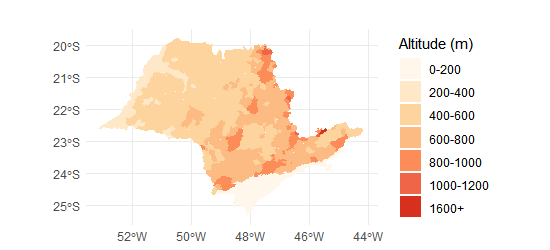
\includegraphics[height = 5cm]{Imagens/M01.png}
\\{\scriptsize Figura 22. Distribuição espacial dos municípios do estado de São Paulo em classes segundo a altitude (m) de sua sede.}
\end{figure}

\begin{resposta}
A distribuição de altitude no estado se dá de maneira regular. Ainda, a maior parte dos municípios se apresenta em uma faixa específica dentre os valores determinados.
\end{resposta}

\subsection {Área}

\begin{figure}[h!]
\centering
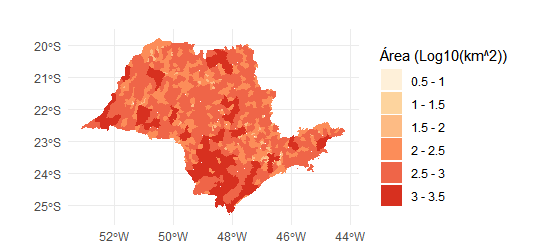
\includegraphics[height = 5cm]{Imagens/M02.png}
\\{\scriptsize Figura 23. Distribuição espacial dos municípios do estado de São Paulo em classes segundo a área (Log10 km2).}
\end{figure}

\begin{resposta}
A distribuição do $\log_{10}$ da área, também é regular. Há uma quantidade limitada de municípios com áreas muito baixas, ou seja, os outliers.
\end{resposta}


\subsection {População}

\newpage

\begin{figure}[h!]
\centering
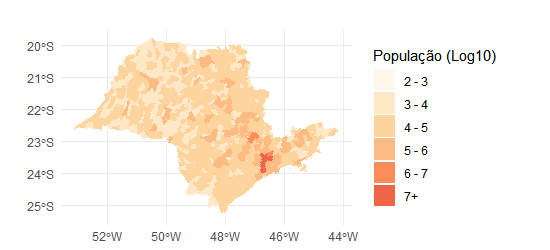
\includegraphics[height = 5cm]{Imagens/M03.png}
\\{\scriptsize Figura 24. Distribuição espacial dos municípios do estado de São Paulo em classes segundo o tamanho da população humana (Log10 indivíduos).}
\end{figure}

\begin{resposta}
A distribuição do $\log_{10}$ da população também é regular, a cidade de São Paulo é um outlier evidente no mapa.
\end{resposta}

\subsection {Registros}

\begin{figure}[h!]
\centering
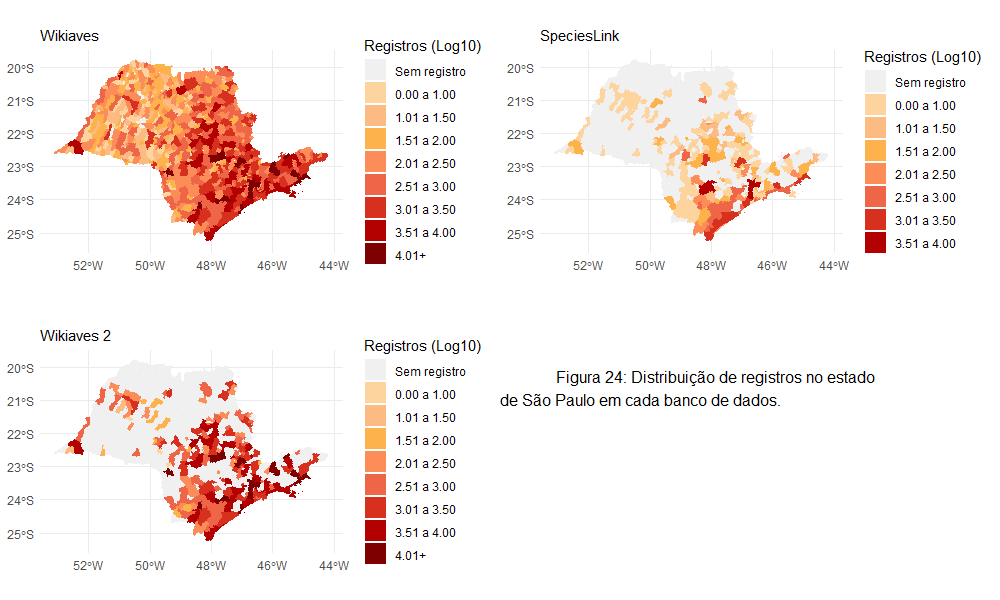
\includegraphics[width=17cm]{Imagens/M04.png}
\\{\scriptsize Figura 25. Distribuição espacial dos municípios do estado de São Paulo em classes segundo o número de registros (Log10, esquerda) e o número de espécies (Log10, direita) em cada banco de dados (WAV = superior, SLI = central, WAV2 = inferior).}
\end{figure}

\begin{resposta}
Há uma desigualdade perceptível entre os bancos de dados quanto a distribuição espacial da quantidade de registros. O mapa do Wikiaves é mais saturado que o do SpeciesLink, a quantidade de cidades sem registro, também, torna-se ainda mais evidente: enquanto o Wikiaves cobre quase todo o estado, o SpeciesLink não cobre metade disto. 

Não obstante, há similaridades observadas nos mapas, eles mostram uma expressão mais forte no litoral e, conforme se movimenta para  o interior há uma diminuição na quantidade de registros, enfatizando a relevância dos parâmetros de latitude e longitude.
\end{resposta}

\subsection {Espécies}

\begin{figure}[h!]
\centering
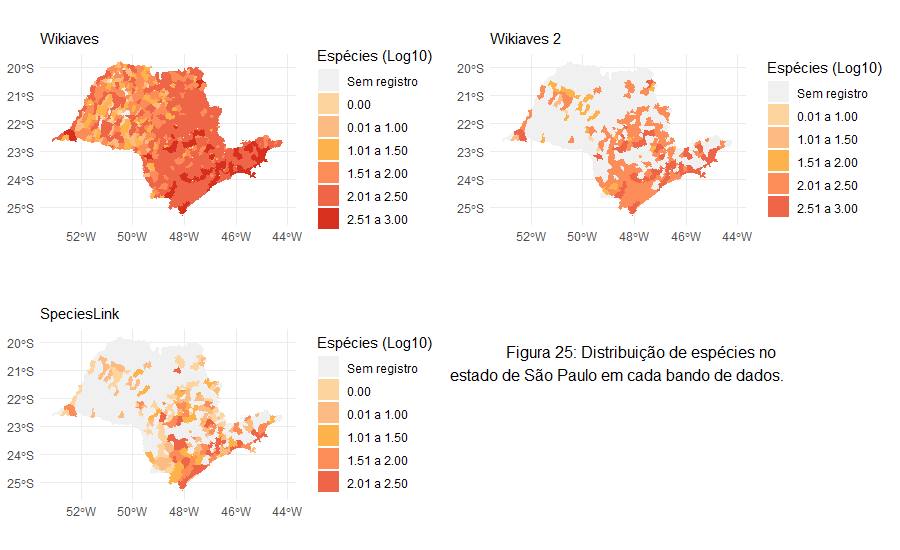
\includegraphics[width=17cm]{Imagens/M05.png}
\end{figure}

\begin{resposta}
As mesmas divergências e semelhanças mencionadas na subseção anterior são encontradas para a quantidade de espécies, de forma menos chamativa. 
\end{resposta}